\subsection[ Assorbimento, diffusione di onda E.M.]{Descrivere qualitativamente il fenomeno dell'assorbimento, il fenomeno della diffusione elastica ed il fenomeno della diffusione inelastica di un'onda e.m. su un sistema.}
Schematizzando il sistema come una scatola su cui facciamo incidere onde e.m. e osservando la radiazione emessa dall'oggetto pssiamo distinguere tre fenomeni:
\begin{figure}[H]
	\centering
	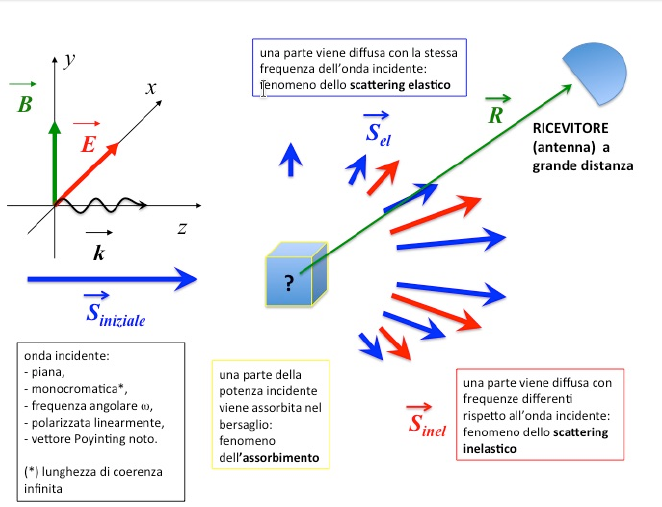
\includegraphics[width=0.4\textwidth]{immagini/1.png}
	\caption{Assobimento e diffusione e.m. di un sistema}
	\label{fig:1}
\end{figure}
Una parte della potenza irraggiata dall'onda sorgente può essere assorbita dall'oggetto (quindi dissipata con qualche meccanismo interno): fenomeno dell'assorbimento.\\
Una parte della potenza dell'onda incidente può essere diffusa sempre con la medesima frequenza: fenomeno della diffusione elastica.\\
Una parte della potenza dell'onda incidente può essere diffusa con frequenze differenti dalla incidente stessa: fenomeno della diffusione inelastica.\\
Un esempio di sistema di questo tipo è l'atomo in cui l'onda incidente eccita gli elettroni che, accelerando, possono irraggiare e dare luogo ai tre fenomeni citati.

\subsection[ Sezioni d'urto di onda E.M. su bersaglio]{Per un’onda e.m. monocromatica che incide su un bersaglio (per esempio un circuito o un atomo) definire le sezioni d’urto: di assorbimento, elastica differenziale, totale elastica; inelastica differenziale; inelastica totale; totale.}
\begin{itemize}
\item Sezione d'urto di assorbimento: 
	\[
		\sigma_{abs} = \frac{\left< P_{abs} \right> }{\left< \left|S_{in}\right| \right> }
	\] 	
\item Sezione d'urto elastica:
	\[
		\sigma_{el} = \frac{\left<P_{el} \right>}{\left< \left| S_{in} \right|  \right>} 
	\] 
	\[
		\frac{\mbox{d} \sigma_{el}}{\mbox{d} \Omega} = R^2 \frac{\left< \left| S_{el}\left( \theta,\phi \right)  \right|\right>}{ \left< \left| S_{in} \right|  \right> } 
	\] 
\item Sezione d'urto inelastica:\\
per ogni frequenza angolare $\omega_{i}$ a cui avviene la diffusione si ha:
\[
	\sigma_{\omega_{i}} = \frac{\left<P_{\omega_{i}} \right>}{\left< \left| S_{in} \right|  \right>} 
\] 
\[
	\frac{\mbox{d} \sigma_{\omega_{i}}}{\mbox{d} \Omega} = R^2 \frac{\left< \left| S_{\omega_{i}}\left( \theta,\phi \right)  \right|\right>}{ \left< \left| S_{in} \right|  \right> }
\] 
\item Sezione d'urto totale: 
	\[
	\sigma_{tot} = \sigma_{abs} + \sigma_{el} + \sum_{n=i} \sigma_{\omega_{i}}
	\] 
\end{itemize}
Da notare che l'unità di misura della sezione d'urto è quella di un'area.

\subsection[ Ampiezza di scattering]{Definire la ampiezza di scattering per un’onda e.m. monocromatica che incide su un bersaglio fisso (per esempio un circuito o un atomo).}
Per uno stato finale del sistema (con l'onda diffusa generata dal bersaglio) a grandi distanze il campo elettrico può esser scritto come il prodotto di un'onda sferica e di un termine che tenga conto della dinamicha del processo:
\[
	\boldsymbol{E}_{f} = \boldsymbol{f}\left( \theta, \varphi \right) \frac{e^{-i\left( \omega_{f}t - k_{f}R + \phi \right)}}{R}
\]
Con $\omega_{f}$ frequenza uscente, $k_{f}$ vettore d'onda uscente, $\phi$ fase.\\
L'ampiezza di scattering $\boldsymbol{f}$ è quindi l'ampiezza dell'onda sferica riemessa dall'oggetto scatterante (che interagisce con un'onda piana monocromatica). Questa è legata alla sezione d'urto differenziale dalla relazione:
\[
	\frac{\mbox{d} \sigma_{\omega_{f}}}{\mbox{d} \Omega} = \frac{\left| \boldsymbol{f}\left( \theta, \varphi \right) \right|^2}{\left| \boldsymbol{E_{0}} \right|^2 }
\] 


\subsection[ Potenza irraggiata da dipolo elettrico, magnetico e quadrupolo elettrico]{Descrivere la situazione in cui la legge 
\[
	P = \frac{2}{3c^3} \ddot{\boldsymbol{p_{e}}}^2 + \frac{1}{180 c^5} \dddot{Q_{ij}}^2 + \frac{2}{3c^3} \ddot{\boldsymbol{p_m}}^2
\] 
(espressa in CGS) è applicabile e spiegare il significato e l'unità di misura di ogni grandezza fisica ivi indicata; trascrivere poi l'espressione in MKSA.}
P è la potenza irraggiata da un sistema in cui sono presenti un dipolo elettrico (1), un quadrupolo magnetico (2) ed un dipolo magnetico (3):
\begin{enumerate}
	\item Dipolo elettrico:
	\[
		P_{1}^{CGS} = \frac{2}{3 c^3} \ddot{\boldsymbol{p}}_{el}^2 \quad \quad 
		P_{1}^{MKS} = k_{0}\frac{2}{3 c^3} \ddot{\boldsymbol{p}}_{el}^2
	\]
	con
	\[
		\boldsymbol{p}_{e} = \sum_{cariche} q \boldsymbol{r} 
	\] 
	\item Quadrupolo elettrico:
	\[
		P_{2}^{CGS} = \frac{1}{180 c^{5}}\dddot{Q_{ij}}^2 \quad \quad 
		P_{2}^{MKS} = k_{0} \frac{1}{180 c^{5}} \dddot{Q_{ij}}^2
	\]
	con
	\[
		\Q = \sum_{cariche}q\left( 3 \boldsymbol{r} \wedge \boldsymbol{r} - \boldsymbol{r}^2\I \right) 
	\] 
	\item dipolo magnetico:
	\[
		P_{3}^{CGS} = \frac{2}{3c^{3}} \ddot{\boldsymbol{p}}_{m}^2 \quad \quad 
		P_{3}^{MKS} = k_{0} \frac{2}{3c^5} \ddot{\boldsymbol{p} }_{m}^2
	\]
	con
	\[
		p_{m} = \frac{1}{2[c]} \sum_{cariche} q \boldsymbol{r} \wedge \boldsymbol{v}   
	\] 
\end{enumerate}
Queste sono applicabili se le dimensioni caratteristiche dell'oggetto che emette sono molto più piccole della lunghezza d'onda incidente. 


\subsection[ Distribuzione angolare della radiazione di dipolo elettrico e magnetico (non relativistico)]{Scrivere la distribuzione angolare della radiazione di dipolo elettrico e di dipolo magnetico nel caso non relativistico.}
\begin{figure}[H]
	\centering
	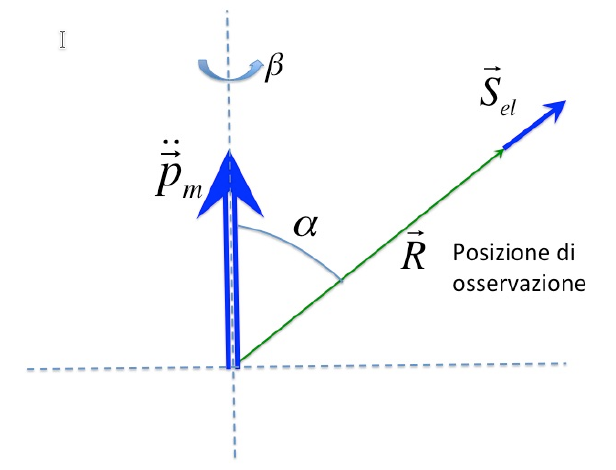
\includegraphics[width=0.4\textwidth]{immagini/2.png}
	\caption{Dipolo magnetico oscillante.}
	\label{fig:2}
\end{figure}
Sulla base della notazione di figura si ha:
\paragraph*{MKSA} I campi e la potenza irraggiata si scrivono come:\\
Dipolo magnetico:
\[
	\boldsymbol{E} = -k_{0}\frac{\ddot{\boldsymbol{p}}_m\left( t_{rit} \right) \wedge \hat{r} }{\left| \boldsymbol{r} \right| c^3} \quad \quad 
	\boldsymbol{B} = k_{0}\frac{\left( \ddot{\boldsymbol{p}}_{m}\left( t_{rit} \right) \wedge \hat{r}  \right) \wedge \hat{r}  }{ \left| \boldsymbol{r}  \right| c^3 }
\] 
\[
	P_m = \frac{\left| \ddot{\boldsymbol{p} }_{m} \right|^2}{6 \pi \epsilon_0 c^5} \quad  \quad \quad 
	\frac{\mbox{d} P_{m} }{\mbox{d} \Omega} = \frac{\mbox{d} P_m}{\mbox{d} \cos{\alpha \mbox{ d}\beta}} = \frac{1}{16 \pi ^2 \epsilon_0 c^5} \ddot{\boldsymbol{p}}_m^2( t_{rit})  \sin^2{\alpha} 
\] 
Dipolo elettrico:
\[	
	\boldsymbol{E} = k_{0}\frac{\left( \ddot{\boldsymbol{p}}_{e}\left( t_{rit} \right) \wedge \hat{r}  \right) \wedge \hat{r}  }{ \left| \boldsymbol{r}  \right| c^2 } \quad \quad 
	\boldsymbol{B} = k_{0}\frac{\ddot{\boldsymbol{p}}_e\left( t_{rit} \right) \wedge \hat{r} }{\left| \boldsymbol{r} \right| c^2} 
\] 
\[
	P_e = \frac{\left| \ddot{\boldsymbol{p} }_{e} \right|^2}{6 \pi \epsilon_0 c^3} \quad  \quad \quad 
	\frac{\mbox{d} P_{e}}{\mbox{d} \Omega} = \frac{\mbox{d} P_e}{\mbox{d} \cos{\alpha \mbox{ d}\beta}} = \frac{1}{16 \pi ^2 \epsilon_0 c^3} \ddot{\boldsymbol{p}}_e^2( t_{rit})  \sin^2{\alpha} 
\] 
\paragraph*{CGS} I campi e la potenza irraggiata si scrivono come:\\
Dipolo magnetico:
\[
	\boldsymbol{E} = -\frac{\ddot{\boldsymbol{p}}_m\left( t_{rit} \right) \wedge \hat{r} }{\left| \boldsymbol{r} \right| c^2} \quad \quad 
	\boldsymbol{B} = \frac{\left( \ddot{\boldsymbol{p}}_{m}\left( t_{rit} \right) \wedge \hat{r}  \right) \wedge \hat{r}  }{ \left| \boldsymbol{r}  \right| c^2 }
\] 
\[
	P_m = \frac{2}{3}\frac{\left| \ddot{\boldsymbol{p} }_{m} \right|^2}{c^3} \quad \quad \quad 
	\frac{\mbox{d} P_{m} }{\mbox{d} \Omega} = \frac{\mbox{d} P _m}{\mbox{d} \cos{\alpha \mbox{ d}\beta}} = \frac{1}{4 \pi c^3} \ddot{\boldsymbol{p}}_m^2( t_{rit})  \sin^2{\alpha} 
\] 
Dipolo elettrico:
\[	
	\boldsymbol{E} = \frac{\left( \ddot{\boldsymbol{p}}_{e}\left( t_{rit} \right) \wedge \hat{r}  \right) \wedge \hat{r}  }{ \left| \boldsymbol{r}  \right| c^2 } \quad \quad 
	\boldsymbol{B} = \frac{\ddot{\boldsymbol{p}}_e\left( t_{rit} \right) \wedge \hat{r} }{\left| \boldsymbol{r} \right| c^2} 
\] 
\[
	P_e = \frac{2}{3}\frac{\left| \ddot{\boldsymbol{p} }_{e} \right|^2}{c^3} \quad \quad \quad 
	\frac{\mbox{d} P_{e}}{\mbox{d} \Omega} = \frac{\mbox{d} P_e}{\mbox{d} \cos{\alpha \mbox{ d}\beta}} = \frac{1}{4 \pi c^3} \ddot{\boldsymbol{p}}_e^2( t_{rit})  \sin^2{\alpha} 
\]
Si potrebbe fare una verifica con: 
\[
	P = \int{ \frac{\mbox{d} P}{\mbox{d} \Omega}} \text{d}\Omega
\] 
\subsection[ Resistenza di irraggiamento per un circuito ad una maglia]{Definire la "resistenza di irraggiamento" di un circuito elettrico a una maglia e fornire un esempio.}
Nota la corrente ($I$) che scorre nel circuito la resistenza di irraggiamento è la resistenza dovuta alla dissipazione per irraggiamento:
\[
	R_{irr} = \frac{P_{irr}}{I^2}
\] 
Ad esempio per un circuito planare si ha (CGS):
\[
	\boldsymbol{m}  = IS \hat{n} / c \implies 
	R_{irr} = \frac{2}{3}\frac{S^2\omega^{4}}{c^{5}}
\] 

\subsection[ Urto elastico ed inelastico tra particelle con esempi]{Definire urto elastico ed urto inelastico fra due particelle; fornire poi almeno un esempio di reazione elastica ed una inelastica fra: 
	\begin{enumerate}
		\item un fotone ed un atomo
		\item due particelle cariche
		\item un protone ed un nucleo.
	\end{enumerate}
}
Un urto è elastico se la natura delle particelle non varia nell'urto stesso, ovvero se per ogni costituente
\[
	p^{\mu}_{i}p_{i,\mu} = m_{i}^2
\] 
è costante nel tempo. Urti di questo tipo sono della forma:
\[
	a \ + \ b \implies a \ + \ b
\] 
In tutti gli altri casi l'urto è anaelastico e si hanno situazion del tipo:
\[
	a \ + \ b \implies \sum_{i} p_{i}
\] 
Diamo adesso esempi di reazioni:
\paragraph{Fotone e Atomo}
\begin{itemize}
	\item Elastico: Scattering Thomson. 
	\[ 
		\gamma \ + \ H \implies \gamma \ + \ H 
	\]
	\item Inelastico: Effetto Compton.
	\[
		\gamma \ + \ A \implies \gamma \ + \ e^- \ + \ A^+
	\] 
\end{itemize}
\paragraph{Due particelle cariche}
\begin{itemize}
	\item Elastico: 
	\[
		p \ + \ p \implies p \ + \ p 
	\] 
	\item Inelastico: Produzione del bosone di Higs
	\[
		p \ + \ p \implies H \ + \ \ldots
	\] 
\end{itemize}
\paragraph{Protone e Nucleo}
\begin{itemize}
	\item Elastico: 
	\[
		\text{da trovare ancora\ldots}
	\]
	\item Inelastico: Reazione degli alchimisti
	\[
		p \ + \ {}^{198}_{80}\text{Hg}_{118} \implies p \ + \ p \ + \ {}^{197}_{79}\text{Au}^{-}_{118} 
	\] 
\end{itemize}
\subsection[ Conservazione di alcune grandezze per interazioni elettromagnetiche/forti]{Dire quali fra le seguenti grandezze si conservano sempre nei processi di urto in cui avvengano interazioni elettromagnetiche e/o forti, ma non deboli.} 
\begin{enumerate}
	\item \textbf{carica elettrica.} Si conserva.
	\item \textbf{numero barionico.} Si conserva.
	\item \textbf{numero leptonico elettronico.} Si conserva. 
	\item \textbf{numero leptonico muonico.} Si conserva.
	\item \textbf{numero di elettroni.} Non si conserva: Formazione di coppie.
		\[
			\ce{ \ce{\gamma} -> \ce{e^+} + \ce{e^-}}
		.\]  
	\item \textbf{differenza fra il numero di elettroni ed il numero di positroni.} Si conserva.
	\item \textbf{numero di protoni.} Non si conserva: produzione di protoni su nucleo.
	\item \textbf{differenza fra il numero di protoni ed il numero di antiprotoni.} Si conserva.
\end{enumerate}


\subsection[ Conservazione di alcune grandezze per interazioni forti]{Dire quali fra le seguenti grandezze si conservano sempre nei processi di urto in cui avvengano esclusivamente interazioni forti:  Fornire almeno un esempio per ogni situazione in cui vi sia una grandezza non conservata.}
\begin{enumerate}
	\item \textbf{carica elettrica.} Si conserva.
	\item \textbf{numero barionico.} Si conserva.
	\item \textbf{numero leptonico elettronico.} Si conserva.
	\item \textbf{numero leptonico muonico.} Si conserva.
	\item \textbf{numero di elettroni.} Si conserva.
	\item \textbf{differenza fra il numero di elettroni ed il numero di positroni.} Si conserva.  
	\item \textbf{numero di protoni.} Si conserva.
	\item \textbf{differenza fra il numero di protoni ed il numero di antiprotoni.} Si conserva.
\end{enumerate}


\subsection[$\ $ Conservazione di alcune grandezze per interazioni deboli]{Dire quali fra le seguenti grandezze si conservano sempre nei processi di urto in cui avvengano interazioni deboli, fornire almeno un esempio quando si ha qualcosa di non conservato.}
\begin{enumerate}
	\item \textbf{carica elettrica.} si conserva.
	\item \textbf{numero barionico.} si conserva.
	\item \textbf{numero leptonico elettronico.} non si conserva.
	\[
		\mu^- \implies e^- \ + \ \gamma
	\]
	\item \textbf{numero leptonico muonico.} Non si conserva, stessa interazione di sopra.
	\item \textbf{numero di elettroni.} Non si conserva: Decadimento del Neutrone.
	\[
		n \implies p \ + \ e^- \ + \ \overline{\nu}_{e}
	\] 
	\item \textbf{differenza fra il numero di elettroni ed il numero di positroni.} Non si conserva: Decadimento $\beta^+$
	\[	
		\ce{\ce{^{A}_{Z}X_{N}} -> \ce{^{A}_{Z-1}Y^{-}_{N+1}} + e^{+} + \nu_{e} }
	\] 
	\item \textbf{numero di protoni.} Non si conserva: Decadimento $\beta^-$
	\[
		\ce{\ce{^{A}_{Z}X_{N}} -> \ce{^{A}_{Z+1}Y^{+}_{N-1}} + e^{-} + \overline{\nu}_{e} }
	\] 
	\item \textbf{differenza fra il numero di protoni ed il numero di antiprotoni.} Non si conserva: Decadimento $\beta^-$ 
\end{enumerate}

\subsection[$\ $ Processi esclusivi e inclusivi, esotermici e endotermici, Q-value.]{Definire i processi esclusivi e inclusivi, il Q-valore di un processo e i processi esotermici o endotermici.}
Un processo si dice esclusivo se in esso viene misurato il 4-impulso di tutti i prodotti. Un processo si dice inclusivo se in esso vengono misurati solo i 4-impulsi di alcuni prodotti.\\
Il Q-valore di un processo è definito come: 
\[
	Q = \left( m_{i} - m_{f} \right) c^2 = T_f - T_i
\] \label{eq:Q-valore}
Un processo è esotermico se $Q > 0$, endoterimco altrimenti.

\subsection[$\ $ Tre definizioni di sezione d'urto equivalenti nei processi corpuscolari]{Definire la sezione d’urto nei seguenti tre casi, e dimostrare come da ognuno di essi si possano dedurre gli altri due: 
\begin{enumerate}
	\item Particelle incidenti su un unico bersaglio [dati: $j_{\text{incidenti}}$; $N_f$] 
	\item Sottile fascio di particelle incidenti su una lastra contenente i bersagli [dati: $\Phi_{incidenti}$, $\hat{\sigma}_{bersagli}$, $N_f$] 
	\item Urti nel volume fra particelle di due specie diverse e differenti concentrazioni [dati: $N_{eventi}$ per unità di tempo e di volume, $n_1$ e $n_2$ concentrazione delle particellle interagenti, $v_{rel}$ (si ipotizza che tutte le particelle di una specie abbiano la stessa velocità).]
\end{enumerate}
Con $\hat{\sigma}$ densità superficiale di eventi,  $j$ densità di corrente, $N_f$ frequenza di eventi osservati (o numero di eventi per unità di tempo),  $\Phi$ flusso di particelle. 
}
Nel primo caso si ha:
\[
	\sigma = \frac{1}{\left| \boldsymbol{j}\right|} \frac{\mbox{d} N_{f}}{\mbox{d} t} 
\] 
Nel secondo invece:
\[
	\sigma = \frac{1}{n_s \Phi} \frac{\mbox{d} N_f}{\mbox{d} t} 
\] 
Nel terzo:
\[
	\sigma = \frac{1}{n_1 n_2 v_{rel}} \frac{\mbox{d} n_f}{\mbox{d} t} 
\] 
Nell'ultimo la sezione d'urto dipende dalla velocità relativa. Inoltre se si ha la funzione di distrubuzione per la velocità relativa:
\[
	\frac{\mbox{d} N_f}{\mbox{d} t} = n_1 n_2 \int_0^\infty \sigma\left( v_{rel} \right) f\left( v_{rel} \right) dv_{rel}
\] 
Per passare dal primo al secondo caso basta osservare che:
\[
	\Phi = \left| \boldsymbol{j} \right| S, \quad \quad 
	n_{s} = \frac{1}{S} \quad \left( \text{un bersaglio} \text{} \right) 
\] 
Con S area del bersaglio.
Se mi metto in un sistema in cui una delle particelle è ferma, è evidente mostrare l'equivalenza tra il caso (2) e (3).

\subsection[$\ $ Sezione d'urto elastica, inclusiva, esclusiva e totale per urti tra particelle]{Per gli urti fra due particelle definire le sezioni d'urto: elastica, inelastica, inclusiva, esclusiva, totale.}
Consideriamo la reazione:
\[
	a \ + \ b \implies p_1 \ + \ p_2 \ + \ \ldots \ + \ p_n
\] 
e sia $f_i\left( E_i \right) $ la distrubuzione di probabilità dell'energia del prodotto i-esimo. La sezione d'urto inclusiva di tale prodotto è:
\[
	\sigma_i = \int_{E_{i, min}}^{E_{i,max}} f\left( E_{i} \right) dE_{i}
\]
Se invece si considera la distribuzione degli impulsi di tutte le particelle finali: $f\left( P_{1}, \ldots , P_{n} \right) $ si ha una sezione d'urto esclusiva:
\[
	\sigma_e = \int f\left( P_{1}, \ldots P_{n} \right) \prod_{i = 1}^{n}d^{4}P_i  
\] 
La sezione d'urto elastica è la sezione d'urto reltiva as un urto elastico, la sezione d'urto anaelastica è la sezione d'urto relativa ad un urto anaelastico.

\subsection[$\ $ Probabilità di interazione di particella su lamina sottile]{Calcolare la probabilità di interazione per una particella che incide su una lamina sottile [dati: $\sigma$ processo, $N_{bersagli}$ per unità superficie].\\
Che significato avrebbe una probabilità maggiore di uno? Quest'ultima risposta dipende dalle tipologie degli urti?}
La probabilità di interazione è: $P = N \sigma $. Se  questa è maggiore di 1 significa che è venuta meno l'approssimazione di lamina sottile. In ogni caso questa non dipende dal tipo di interzaione.

\subsection[$\ $ Forza di reazione radiativa]{Indicare le condizioni per cui la forza di reazione radiativa per una particella (di massa m e carica unitaria) $F_{rad} = m \tau \dot{\boldsymbol{a}}$ è da considerarsi valida ed utilizzabile.} \label{subsec: 2.a.15}
Si ritiene necessario, per indicare le approssimazioni, ricavare la forza in questione. 
La forza di radiazione può essere defita come la forza il cui lavoro è responsabile della perdita di energia per irraggiamento noto nella formula di Larmor (CGS):
\[
	\int_{t_1}^{t_2} \boldsymbol{F}_{rad} \cdot \boldsymbol{v} dt = -\frac{2}{3} \frac{e^2}{c^3} \int_{t_1}^{t_2} \dot{\boldsymbol{v}}^2
\]
Posso scrivere:
\[
	\dot{\boldsymbol{v}}^2 = \frac{\mbox{d} \left( \boldsymbol{v} \dot{\boldsymbol{v}} \right) }{\mbox{d} t} - \boldsymbol{v} \ddot{\boldsymbol{v}} 
\]
Inserendo nel secondo membro della equazione si ha:
\[
	\int_{t_1}^{t_2}{ \boldsymbol{F_{rad}} \cdot \boldsymbol{v} dt } = -
\left. \frac{2}{3}\frac{e^2}{c^3} \boldsymbol{v} \cdot \dot{\boldsymbol{v}}\right|_{t_{1}}^{t_{2}} + \frac{2}{3}\frac{e^2}{c^3} \int_{t_1}^{t_2} \boldsymbol{v}  \cdot \ddot{\boldsymbol{v}} dt
\] 
Se il moto è periodico di ha: 
\[
	\int_{t_1}^{t_2} \left( \boldsymbol{F}_{rad} - \frac{2}{3}\frac{e^2}{c^3}\ddot{\boldsymbol{v}} \right) \cdot \boldsymbol{v} dt = 0  
\] 
Poiche velocità e accelerazione sono ortogonali in tal caso, abbiamo quindi un candidato per la $\boldsymbol{F}_{rad}$.
\[
	\boldsymbol{F}_{rad} = \frac{2}{3}\frac{e^2}{c^3} \ddot{\boldsymbol{v}}.  
\] 
che in MKSA si scrive come:
\[
	\boldsymbol{F}_{rad} = \frac{q^2}{6\pi \epsilon_0 c^3} \dddot{\boldsymbol{x}} = m_{e}\frac{q^2}{6\pi \epsilon_0 c^3} \dddot{\boldsymbol{x}} = m_e \frac{2}{3}\frac{r_e}{c} \dddot{\boldsymbol{x}} = m_e \tau \dddot{\boldsymbol{x}} 
.\] 
Possiamo quindi dare una stima dei valori tipici di questa forza:
\[
r_e = \frac{q^2}{4\pi \epsilon_0 m_e c^2} = 2.82 fm \implies \tau = \frac{2}{3}\frac{r_e}{c} = 6.2 \cdot 10^{-24} s 
.\] \label{eq: raggio classico} 
Tenendo conto della forza viscosa che agisce classicamente sull'elettrone 
\[
	\boldsymbol{F}_{visc} = -\beta \dot{\boldsymbol{x}} = - m_e \Gamma' \dot{\boldsymbol{x}} 
\]
con valori tipici: $\Gamma' \sim 10^{10} \ s^{-1}$.\\
Infine ipotizzando anche una forza "elastica" attrattiva nucleare con valore tipoco $\omega_{0} \sim 10^{14} - 10^{16}$ otteniamo la relazione:
\[
\Gamma' \ll \omega_{0} \ll \frac{1}{\tau}
.\] \label{eq:relazione-parametri-elettrone} 
Questo conto sarà utile per la Domanda \hyperref[subsec: 2.b.12]{2.b.12}.

\subsection[$\ $ Significato fisico della Breight-Wiegner]{Spiegare il significato e indicare l'unità di misura di ogni grandezza fisica nelle seguenti leggi:
\[
	\left( 1 \right) \to \frac{\mbox{d} \sigma_{el}}{\mbox{d} \Omega} = r_{e}^2 L \left( \omega \right)  \sin^2 \left( \alpha \right)   \quad \quad
	\left( 2 \right) \to  \frac{\mbox{d} \sigma_{el}}{\mbox{d} \Omega} = r_{e}^2 L \left( \omega \right)  \frac{1 + \cos^2 \left( \alpha \right) }{2}   
\]
\[
	\left( 3 \right) \to  \sigma_{el} = \sigma_{Th} L \left( \omega \right) \quad \quad 
	\left( 4 \right) \to  \sigma_{tot} = 4 \pi r_{e} c \frac{\omega^2 \Gamma }{\left( \omega_{0}^2 - \omega^2 \right)^2 + \omega^2 \Gamma_{tot} } 
\] 
con 
\[
	L \left( \omega \right) = \frac{\omega^4}{\left( \omega_{0}^2 - \omega^2 \right)^2 + \omega^2 \Gamma_{tot} } \quad \quad 
	\sigma_{Th} = \frac{8}{3} \pi r_{e}^2 = 0.66 \text{ barn}
\]
inerenti l'interazione di un’onda e.m. piana e monocromatica su un elettrone legato elasticamente.} \label{subsec: 2.a.16}
L'equazione (1) è la sezione d'urto differenziale per l'interazione tra l'elettrone ed un onda polarizzata linearmente. Può essere ottenuta dalla equazione del moto dell'elettrone legato elasticamente soggetto alle forze della domanda precedente (di richiamo, di attrito viscoso e radiazione radiativa) immerso nel campo di una onda e.m. piana monocromatica (vedi Domanda \hyperref[subsec: 2.b.12]{2.b.12}):
\[
	\boldsymbol{x} = \frac{e \boldsymbol{E_0}}{m_e}\frac{1}{\omega_0^2-\omega^2- i\omega \Gamma' - i \tau \omega^2} = \frac{eE_0}{m_e}\frac{1}{\omega_0^2-\omega^2- i\omega\Gamma_{tot}}
.\] 
In cui si definiscono 
\[
	\Gamma_{tot} = \Gamma' + \Gamma \frac{\omega^2}{\omega_0^2} \quad \quad 
	\Gamma = \omega_0^2 \tau \quad \text{ con $\tau$ quello ottenuto nella domanda precedente}
\]
Quindi basta adesso ricordare che la distribuzione angolare di potenza irraggiata da un dipolo oscillante $ \boldsymbol{p} = \boldsymbol{p}_0 e^{-i\omega t}$ è:
\[
	\frac{\mbox{d} P}{\mbox{d} \Omega} = \frac{\omega^{4} \left| \boldsymbol{p}_0 \right|^2 }{4\pi c^3} \sin^2\left( \alpha \right) 
.\] 
Quindi inserendo $\left| \boldsymbol{p}_0 \right| = \left| e \boldsymbol{x} \right| $  e dividendo per il vettore di Poynting incidente si ha la tesi (1).

L'equazione (2) è la sezione d'urto differenziale con l'onda incidente non polarizzata: bisogna in questo caso mediare su tutte le possibili polarizzazioni dell'onda incidente ottendendo il fattore finale.\\
l'espressione (3) si ottinene integrando sull'angolo solido la (1) o la (2).\\
infine la (4) è la sezione d'urto totale definita come:
\[
	\sigma_{tot} = \frac{e \left< \dot{\boldsymbol{x}}\boldsymbol{E}\right>}{\left<\boldsymbol{S_{in}} \right>}
.\]
Possiamo notare anche che:
\[
	\frac{\sigma_{el}}{\sigma_{tot}} = \frac{1}{1 + \Gamma'/\left( \omega^2\tau \right)  }
.\] 
Che tende all'unità quando non c'è dissipazione.

\subsection[$\ $ osservazioni sullo scattering Rutherford]{Discutere qualitativamente le osservazioni sperimentali dello scattering di Rutherford.}
Inviando un fascio di particelle $\alpha$ su una lamina d'oro si osserva che circa 1 particella su 8000 viene deviata a grandi angoli o rimbalza. Queste osservazioni non sono spiegabili con il modello a panettone di Thomson ma si spiegano bene con il modello di Bhor.
\[
	\left. \frac{\mbox{d} \sigma}{\mbox{d} \Omega} \right|_{Ruth} = \frac{1}{\left(4\pi \epsilon_0\sin^{2}\left( \frac{\theta}{2} \right) \right)^2 } \left(\frac{zZe^2}{4T} \right)^2 
.\] 
Si deduce facilmente che le particelle più energetiche sono più penetranti, le particelle più cariche vengono maggiormente deflesse.

\subsection[$\ $ Differenza tra Scattering Rutherford e Mott]{Spiegare la differenza fra lo scattering Rutherford e lo scattering Mott.}
Lo Scattering Mott:
\[
	\left. \frac{\mbox{d} \sigma}{\mbox{d} \Omega} \right|_{Mott} = \left. \frac{\mbox{d} \sigma}{\mbox{d} \Omega} \right|_{Ruth} \left( 1- \beta^2 \sin^2\left( \frac{\theta}{2} \right)  \right) 
.\] 
Tiene conto dello spin degli elettroni e degli effetti relativistici che questi hanno nel loro moto.

\subsection[$\ $ Significato dei termini nelle sezioni d'urto Mott e Rutherford]{Spiegare il significato di tutti i termini delle seguenti espressioni delle sezioni d’urto differenziali Rutherford e Mott: 
\[
	\left. \frac{\mbox{d} \sigma}{\mbox{d} \Omega} \right|_{Ruth} = \left( \frac{zZe^2}{4 \pi \epsilon_0} \right)^2 \left( \frac{1}{4T} \right)^2 \frac{1}{\sin^4\left( \theta/2 \right) }  
\] 
\[
	\left. \frac{\mbox{d} \sigma}{\mbox{d} \Omega} \right|_{Mott} = \left. \frac{\mbox{d} \sigma}{\mbox{d} \Omega} \right|_{Ruth} \left( 1 - \beta^2 \sin^2 \theta/2  \right) \quad \quad
	\text{con } T \to \frac{pV}{2}
\] 
}
Sono tutti termini di banale comprensione, ricordiamo però che $\theta$ è l'angolo di scatterig: l'angolo tra la direzione iniziale della particella e quello finale.

\subsection[$\ $ Definizione di raggio nucleare tramite lo Scattering Rutherford]{Dare la definizione operativa di raggio nucleare mediante lo scattering di Rutherford.}
Fissando un angolo di scatternig $\hat{\theta} = 60^o$ si ha che per energie maggiori di $T_{soglia} \approx 30 MeV$ divena importante l'interzione forte con il nucleo: si ha un discostamento dalla legge che lega la sezione d'urto Rutherford a T. Quindi possiamo ipotizzare che la distanza minima che si ottiene in questo caso sia una buona stima del raggio nucleare.
\[
	d \approx 2\cdot \frac{zZ e^2}{4 \pi \epsilon_0 T_{soglia}} \implies R = \frac{d}{2}\left( 1 + \frac{1}{\sin\left( \frac{\hat{\theta}}{2} \right) } \right) 
.\] 
È necessario notare che $R$ è la distanza tra i nuclei degli atomi coinvolti nello scattering, non il nucleo dell'atomo (che vorremmo definire), è quindi necessario incidere con particelle il cui nucleo sia di dimensioni attese molto inferirori rispetto a quelle del nucleo in esame per dare una buona stima del raggio di quest'ultimo (ipotesi verificata nel caso di particelle $\alpha$ su Piombo, ad esempio).

\subsection[$\ $ Definizione di A, Z, N, nuclei isotopi, isobari, isotoni, stabili ed instabili]{Definire le quantità che in un nucleo usualmente si indicano con A, Z, N (simbologia ${}^A_Z X_N$ ). Dare la definizione di nuclei isotopi, isobari, isotoni, stabili, instabili.}
A è il numero di nucleoni (protoni e neutroni), Z è il numero di protoni, N è il numero di neutroni.\\
Due nuclei sono:
\begin{itemize}
	\item Isotopi: hanno lo stesso Z.
	\item Isobari: hanno lo stesso A.
	\item Isotoni hanno lo stesso N.
	\item Instabili: hanno vita media finita.
	\item Stabili: hanno vita media "infinita".
\end{itemize}

\subsection[$\ $ Unità di massa atomica, energia di legame B e difetto di massa $\Delta$]{Dopo avere definito l’unità di massa atomica e avere dato il suo valore in MeV/$c^2$, definire l’energia di legame (B) di un atomo ed il “difetto di massa” ($\Delta$) di un atomo.}
\[
	\text{1 u.m.a.} = \frac{1}{12}m\left( {}^{12}_{6}C_{6} \right) = 931.49 \text{ MeV/}c^2 
.\]
La B è l'energia necessaria per separare un nucleone dal suo nucleo.\\
L'energia di legame B di un nucleo X con A nucleoni e Z protoni è:
\[
	B\left( A, Z \right) = Z\left( m_p + m_e - m_u \right) + N \left( m_n - m_u \right) - \Delta_{A, Z} = 7.29 \text{MeV} \cdot Z + 8.07 \text{MeV} \cdot N - \Delta_{A,Z} 
.\] 
Dove 
\[
	m_u = 1 \text{ u.m.a.}\quad \quad 
	m_p = 938.2 \text{ MeV/}c^2\quad \quad 
	m_e = 0.511 \text{ MeV/}c^2
\]
Il difetto di massa è invece:
\[
	\Delta = m_{x} - \frac{A}{12}m\left( {}^{12}_{6}C_{6} \right) = m_x - Am_u 
.\] 
E lo si pio trovare nelle tabelle in rete.\\
Il difetto di massa è particolarmente utile per ricavare il Q-valore: è immediato esprimere la massa del nucleo coinvolto in una interazione mediante tale quantita e l'unità di massa atomica $m_u$.

\subsection[$\ $ Formula semiempirica B e termini spiegati dal modello a goccia]{Enunciare la formula semiempirica B = B(A,Z) ed indicare i suoi termini che sono spiegati dal modello a goccia. Spiegare le ipotesi su cui tale modello è basato e
fornire l'ordine di grandezza dell’energia media di legame di un nucleone all’interno di un nucleo.}
Nel modello a goccia si ha in prima approssimazione (per nuclei abbastanza grandi) una energia di legame proporzionale al numero di nucleoni e quindi al volume del nucleo stesso:
\[
	B_1\left( A, Z \right) = a_V A \quad \quad \text{Termine correttivo di volume}
.\] 
In seconda approssimazione possiamo considerare che i nucleoni che si trovano sulla superficie del nucleo non sono circondati da altri nucleoni, vi sarà allora un termine correttivo superficiale:
\[
	B_2\left( A,Z \right) = a_S A^{2/3} \quad \quad \text{Termine correttivo di superficie} 
.\] 
Poi possiamo aggiungere una ulteriore correzione per tener conto della repulsione columbiana tra i nucleoni carichi (Z tiene conto della carica, A tiene conto del raggio):
\[
	B_3\left( A,Z \right) = a_C \frac{Z^2}{A^{2/3}} \quad \quad \text{Termine correttivo Columbiano}
.\] 
Si hanno infine altri termini correttivi che tengono di conto di effetti quantistici e del principio di Pauli:
\[
	B\left( A,Z \right) = a_{V}A - a_{S}A^{2/3} - a_{C} \frac{Z^2 }{A^{1/3}} + a_{sym}\frac{\left( Z - N \right)^2}{A} + \delta_{pair} 
.\] \label{eq:B-energy}
Il modello in considerazione è quello "A Goccia", l'ipotesi di questo è che il nucleo di numero atomico Z e peso atomico A occupi un volume sferico di raggio:
\[
	R = r_0 A^{1/3} + r_{skin} \approx \left( 1.25 A^{1/3} + 2.0  \right) fm
.\]
Il modello prevede che l'energia di legame tra due nucleoni sia dell'ordine di $\sim 2.2$ MeV, ovvero la differenza tra la massa del deutone e la somma delle masse del protone e neutrone. 

\subsection[$\ $ Definizione dei decadimenti $\alpha$, $\beta^{+}$,$\beta^{-}$, $\gamma$, cattura elettronica con rispettivi Q-Value]{Definire i decadimenti $\alpha$, $\beta$ , $\gamma$ e il decadimento tramite cattura elettronica in un nucleo. Calcolare il Q-valore per il decadimento $\beta+$, $\beta-$, e per la cattura elettronica a partire dal difetto di massa delle specie coinvolte.} \label{sec:decadimenti}
\paragraph{Decadimento $\alpha$}
\[
	\ce{ \ce{^{A}_{Z}X_{N}} -> \ce{^{A-4}_{Z-2}Y^{2-}_{N-2} + \alpha}} \quad \quad \text{con $\alpha$ nucleo di  \ce{^{4}_{}He^{2+}_{}}}
\]
\paragraph{Decadimento $\beta+$}
\[
	\ce{\ce{^{A}_{Z}X_{N}} -> \ce{^{A}_{Z-1}Y^{-}_{N+1}} + e^{+} + \nu_{e} }
.\]
in cui si ha la transizione:
\[
	\ce{p -> n + e^+ + \overline{\nu}_e}
.\]
Il Q-valore del decadimento è : $Q = \Delta_{A,Z} - \Delta_{A, Z-1} - 2m_e $\\
Il Q-valore della reazione è: $ Q = m_p - m_n - m_e = - 1.804 $MeV.

\paragraph{Decadimento $\beta-$}
\[
	\ce{\ce{^{A}_{Z}X_{N}} -> \ce{^{A}_{Z+1}Y^{+}_{N-1}} + e^{-} + \overline{\nu}_{e} }
.\]
in cui si ha la transizione:
\[
	\ce{n -> p + e^- + \nu_e}
.\]
Il Q-valore del decadimento è : $Q = \Delta_{A,Z} - \Delta_{A, Z+1} $\\
Il Q-valore della reazione di transizione è: $ Q = m_n - m_p - m_e = 0.782 $MeV.
\paragraph{Cattura elettronica}
\[
	\ce{\ce{^{A}_{Z}X_{N}} -> \ce{^{A}_{Z-1}Y_{N+1}} + \nu_e} \quad \quad Q = \Delta_{A,Z} - \Delta_{A, Z-1} 
.\] 
in cui si ha:
\[
\ce{p + e ->n + \nu_e }
.\] 

\subsection[$\ $ Scoperta del neutrino nel decadimento $\beta^{-}$]{Come si e' arrivati alla conclusione che nel decadimento beta deve essere emessa una particella neutra non rivelata? }
Il problema in questione risale al 1934 (con Pauli che ipotizza l'esistenza della particella), venne formalizzato successivamente da Fermi e da Bhor.\\
Ciò che destava sgomento era lo spettro di emissione dell'elettrone. Spieghiamo a grandi linee il problema: \\
All'inzio si pensava che avvenisse il processo
\[
	\ce{n -> p + e-}
.\] 
In cui sicuramente si hanno le relazioni (di qui in avanti c = 1) 
\[
	m_e \text{ (0.511 MeV) }\ll m_p \text{ (938.3 MeV) } \approx m_n \text{ (939.6 MeV)}
.\] 
Conviene quindi ipotizzare che il neutrone si trovi inizialmente fermo, in tal caso anche il protone viene praticamente creato fermo. Per la conservazione dell'energia:
\[
	m_n =E_p + E_e
.\]
con 
\[
	E_p = \sqrt{m_p^2 + p_p^2} \quad \quad 
	E_e = \sqrt{m_e^2 + p_e^2} 
.\]
Se si trascura il rinculo del protone, come ipotizzato sopra:
\[
	m_n \approx m_p + \sqrt{m_e^2 + p_e^2} 
.\]
Quest'ultima relazione fissa l'impulso e l'energia dell'elettrone, quindi ci aspettiamo che lo spettro di quest'ultimo abbia un unico picco, invece sperimentalmente si ottengono curve del tipo:
\begin{figure}[H]
	\centering
	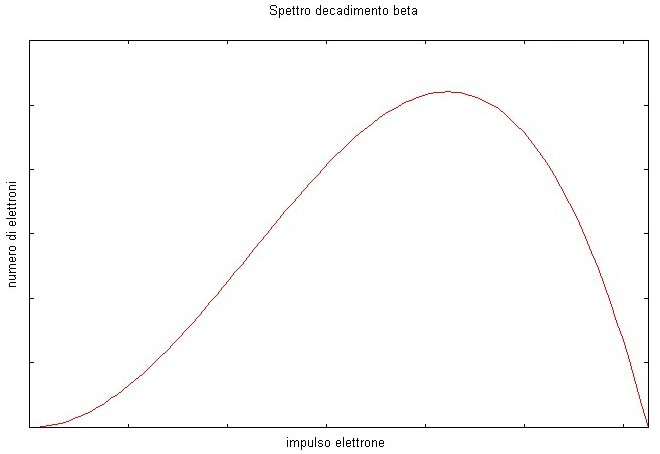
\includegraphics[width=0.5\textwidth]{immagini/Decadimento_beta_(spettro).jpg}
	\caption{Spettro di energia dell'elettrone.}
	\label{fig:beta}
\end{figure} 
Tale grafico mostra uno spettro completo che parte da energie nulle fino ad arrivare ad annullarsi di nuovo a $\sim 5.5 \ m_e$.\\
Per spiegarlo è quindi necessario ipotizzare che vi sia un'altra particella tra i prodotti che è appunto il neutrino.


\subsection[$\ $ Spiegazione dell'esistenza del neutrone nell'atomo]{Spiegare perchè, sebbene il neutrone libero sia instabile, esso non possa decadere quando è all'interno di taluni nuclei.}
Affinchè il neutrone in un nucleo possa decadere è necessario che
\[
	Q = \sum_{in} M_k - \sum_{fin} M_k > 0
.\] 
Questo in alcuni nuclei può non essere verificato, ad esempio:
\paragraph{Stabilità del Deuterio}
\[
	\ce{\ce{^{2}_{1}H_{1}} -> \ce{^{1}_{1}H_{0}} + p + e- + \overline{\nu}_e }
.\] 

con:
\[
	\ce{n -> p + e- + \overline{\nu}_e}
.\] 
si ha che la reazione non avviene perchè: 
\[
	Q = \Delta_{2,1} - 2\Delta_{1,0} = (13.136 -14.578)\text{ MeV} = -1.442 \text{ MeV} 
.\] 

\subsection[$\ $ Particelle per la misura del fattore di forma]{Quali particelle incidenti e di quale energia si utilizzano per misurare i fattori di forma nucleari?}
Si usano in genere Scattering elastici, in particolare la particella adatta è l'elettrone, ad esempio:  
\[
\ce{e- + p  -> e- + p} \quad \quad \text{Per misurare il fattore di forma e.m. del protone}
.\] 
Se funziona con il protone allora funziona anche con i nuclei avendo cura di scegliere le giuste energie con il metodo seguente.\\
Per quanto riguarda l'energia dell'elettrone dobbiamo tener di conto di che lunghezza vogliamo ispezionare: Per sondare oggetti di dimensioni caratteristiche del fm è necessario sondare con energie aventi le stesse dimensioni in termini di lunghezza d'onda di De Broglie:
\[
	E = \hbar \omega = \frac{2\pi\hbar c}{\lambda} =  \frac{1240 \text{ MeV} \cdot \text{fm}}{1 \text{ fm}} = 1240 \text{ MeV}
.\]

\subsection[$\ $ Larghezza di vita media, tempo di dimezzamento, branching fraction]{Dare le definizioni di: larghezza, vita media, semivita (o tempo di dimezzamento), rapporto di decadimento (“Branching fraction” o “Branching ratio”) per il decadimento di una particella.}
Se N è il numero di particelle non ancora decadute la vita media è definita da:
\[
	\dot{N} = -\frac{N}{\tau}
.\] 
La larghezza di vita media è la probabilità di decadimento nell'unità di tempo:
\[
	\Gamma = 1/\tau
.\]
La larghezza viene solitamente espressa in eV tramite:
\[
	\Gamma \text{ [eV]} = \Gamma \text{ [s]}^{-1} \cdot \hbar
.\] 
Perchè una particella che decade si può interpretare come una risonanza piccata nella massa di quest'ultima e di larghezza prorio $\Gamma$.\\
Il tempo di dimezzamento è
\[
	T = \tau \ln\left( 2 \right)  
.\] 
In fine il rapporto di decadimento di un "canale" è il rapporto tra i decadimenti di quel canale ed il numero totale di decadimenti.
\[
	B_{\text{f}} = \frac{\Gamma_{\text{f}}}{\Gamma}
.\] 

\subsection[$\ $ Ordini di grandezza di sezioni d'urto forti o deboli]{ Quali sono gli ordini di grandezza tipici delle sezioni d’urto delle interazioni forti e delle interazioni deboli?}
Per le interazioni forti si hanno sezioni d'urto dell'ordine di $10 - 100$ mb, per le interazioni deboli invece $1$ fb.

\subsection[$\ $ Vite medie per interazioni forti, elettromagnetiche, deboli]{Quali sono, approssimativamente, gli ordini di grandezza delle vite medie dovute ad interazioni deboli, elettromagnetiche, forti?}
\begin{itemize}
	\item Interazioni deboli: dai 15 minuti per il decadimento $\beta$ del neutrone fino a $10^{-8}$ s del decadimento del  $\pi$ carico.
	\item Interazioni eletromagnetiche: tempi tipici sono dell'ordine di $10^{-16}$ s.
	\item Interazione forte: tempi tipici sono $10^{-23}$ s.
\end{itemize}

\subsection[$\ $ Cinematica dell'effetto Mossbauer]{Spiegare la cinematica di un decadimento $\gamma$ nucleare e spiegare qualitativamente l'effetto Mossbauer. }
\paragraph{Definizione di decadimento $\gamma$.}
I decadimenti $\gamma$ sono delle transizioni fra uno stato eccitato di un nucleo ed uno stato di energia inferiore con l'emissione di un fotone (raggi X: 10keV-1MeV).\\
Considerando la reazione:
\[
	\ce{\ce{^{57}_{26}F^*_e} ->[T_{1/2} = 97.7 \text{ ns}] \ce{^{57}_{26}F_e} + \gamma ( 14.4 \text{ keV} ) }
.\] 
\begin{itemize}
	\item $M$: la massa dello stato fondamentale del nucleo.
	\item $M^* = M + E_0$ : la massa dello stato eccitato. 
	\item $E_\gamma$: l'energia del fotone nel laboratorio e nel centro di massa se il decadimento avviene da fermo.	
\end{itemize}
Siamo interessati all'energia dei fotoni uscenti, a prima vista sembrerebbe $E_0$ ma in realtà è una sovrastima: il rinculo del nucleo si porta via energia, vediamolo cinematicamente.\\ 
La quantità di moto del fotone nel centro di massa (e quindi anche dell'atomo di $F_e$):
\[
	E_\gamma = P^\gamma_{cm}
.\] 
Quindi si ha anche che dalla conservazione dell'energia:
\[
	E_{in} = M^* = M + E_0 = E_{fin} = \sqrt{M^2 + E_\gamma^2} + E_\gamma 
.\]
Possiamo quindi ricavare $E_\gamma$ in funzione di tutto il resto:
\[
	E_\gamma = \frac{E_0\left( E_0 + 2M \right)}{2\left( E_0 + M \right)} 
.\]
Essendo la massa del $\ce{^{57}_{26}F_e} = 53.05 \text{ GeV}$ ed $E_0 = 14.4 \text{ keV}$ possiamo approssimare:
\[
	E_\gamma  \approx E_0 - \frac{E_0^2}{2M}
.\] 
Quindi l'energia persa è:
\[
	\Delta E_\gamma \approx - \frac{E_0^2}{2M} \implies \frac{\Delta E_\gamma}{E_\gamma} \approx - \frac{E_0}{2M}  
.\]
Essendo $E_0 \approx E_\gamma$. Nel caso in esame si ha:
\[
	\left| \Delta E_\gamma \right| \approx 1.9 meV \implies \left| \frac{\Delta E_\gamma}{E_\gamma}\right| \approx 1.3 \cdot 10^{-7} 
.\] 
Quest'ultima è molto maggiore di:
\[
	\frac{\Gamma}{E_0} = 3.2 \cdot 10^{-13} 
.\] 
Quindi sarà difficile che un fotone partito dal decadimento riesca ad eccitare un nuovo atomo di $F_e$ poichè il fotone è emesso in un range di energia molto grande rispetto alla larghezza del processo.\\
Se invece prendo un blocco di atomi di ferro (o in gergo: nu bll pezz de ferragl) la massa che va al denominatore nelle equazioni sopra non è più quella del singolo atomo ma quella di tutto il blocco. Succede quindi che:
\[
	\Delta E_\gamma \ll \Gamma 
.\] 
Si può quindi avere un effetto coerente se il fotone che esce urta contro un altro atomo di ferro: Effetto Mosbauer.

\subsection[$\ $ Variabili indipendenti con due reagenti e N prodotti]{Quante sono le variabili indipendenti nello stato finale di una reazione in cui due particelle collidono ed N particelle sono prodotte?}
Sia il processo di decadimento:
\[
	\ce{a + b -> p_1 + p_2 + \ldots \text{+} p_n }
.\] 
Si ha che il numero di osservabili indipendenti è dato da le variabili ed i vincoli in gioco:
\begin{itemize}
	\item n 4-impulsi $\implies$ 4n variabili
	\item n vincoli dovuti alla massa delle singole particelle: $m_i^2 = P_{0, i}^2 - \boldsymbol{P}_{i}^2$
	\item 4 vincoli per la conservazione impulso-energia: $P_{in} = \sum_i P_i$
\end{itemize}
quindi le variabili indipendenti sono 3n - 4.
\paragraph{Nota}%
In quanto affermato non c'è stato bisogno di esplicitare il numero di reagenti, questo numero vale in generale per qualsiasi numero di particelle iniziali (se si hanno n prodotti).

\subsection[$\ $ Variabili indipendenti per un decadimento a due, considerazioni sul caso di Spin nullo]{Quante sono le variabili indipendenti nello stato finale di una reazione in cui una particella decade in due particelle? Quali implicazioni avremmo se la particella che decade avesse un momento angolare nullo? }
Le variabili indipendenti sono 3*2 - 4 = 2, se la particella ha spin nullo allora si ha una isotropia spaziale che ci permette di integrare l'espressione per il decadimento a due corpi:
\[
	\frac{\mbox{d} \Gamma}{\mbox{d} \Omega_1} = f_{dec}\left( \Omega_1 \right) \frac{P_{cm}}{4M} 
.\] 
sull'angolo solido:
\[
	\Gamma = f_{dec} \frac{P_{cm}}{4M}4\pi
.\] 

\subsection[$\ $ Variabili del Dalitz Plot]{Definire le variabili utilizzate nel "Dalitz plot".}
Le variabili del Dalitz plot sono:
\begin{itemize}
	\item $s_{12}$: il quadrato della massa invariante delle particelle 1 e 2
	\item $s_{23}$: il quadrato della massa invariante delle particelle 2 e 3
\end{itemize}

\subsection[$\ $ Variabili indipendenti per il decadimento a tre corpi, considerazioni sul caso di Spin nullo]{Quante sono le variabili indipendenti nello stato finale di una reazione in cui una particella decade in tre particelle? Quali implicazioni avremmo se la particella che decade avesse un momento angolare nullo?}
Le variabili indipendenti sono 3*3-4 = 5.\\
La larghezza di decadimento si può esprimere come:
\[
	\Gamma = \int{f_{dec}\left( s_{12}, s_{23}, \alpha ,\beta,\gamma \right) dL_p}
.\] 
Con $\alpha, \beta,\gamma$ angoli di Eulero e $dL_p$ elemento infinitesimo dello spazio delle fasi definito da:
\begin{align*}
	dL_p &= \frac{\mbox{d}^3 \bs{P}_1}{2E_1}\cdot\frac{\mbox{d}^3 \bs{P}_2}{2E_2}\cdot\frac{\mbox{d}^3 \bs{P}_3}{2E_3}\cdot 
	\delta^4\left(\bs{P}_{\text{in}}- \sum_{n=1}^{3} \bs{P}_i  \right)=\\
	     &= \frac{1}{32s}\text{d}s_{12}\text{d}s_{23}\text{d}\alpha \text{d}\left( \cos\beta \right)\text{d}\gamma 
.\end{align*}
Se la particella ha momento angolare nullo allora lo stato iniziale non ha una direzione privilegiata, quindi $f_{dec}$ non dipende dagli angoli di Eulero e si può integrare su questi ultimi:
\[
	d\Gamma = f_{dec}\left( s_{12}, s_{23} \right) \frac{ds_{12}ds_{23}}{32s} \int_0^{2 \pi}{d\alpha \int_{-1}^1{d\cos\beta \int_0^{2\pi}{ d\gamma }}} = \frac{\pi^2}{4s} f_{dec}\left( s_{12}, s_{23} \right) ds_{12}ds_{23}
.\]
\subsection[$\ $ Funzione di distribuzione esclusiva dei 4-impulsi]{ Definire la funzione di distribuzione esclusiva dei 4-impulsi delle particelle emergenti dopo la collisione di due particelle (oppure dopo il decadimento di una particella).}
Per la collisione di due particelle si ha:
\[
	d\sigma = f_{urto}\left( P_1 \ldots P_n \right)dL_p = f_{urto}\left( P_1 \ldots P_n \right) \frac{\mbox{d}^3 \boldsymbol{P}_1}{2E_1}\ldots \frac{\mbox{d}^3 \boldsymbol{P}_n}{2E_n} \delta^4\left( P_{in}-\sum_{i}P_i \right) 
.\] 
con $\sigma$ sezione d'urto del processo, $f_{urto}$ probabilità di misurare la sezione d'urto $d\sigma$ in un intorno di $P_1 \ldots P_n$ (contenente tutte le informazioni dinamiche del processo) e $dL_p$ è l'elemento infinitesimo dello spazio delle fasi.

\subsection[$\ $ Metodo della massa invariante]{Spiegare il metodo della ‘massa invariante’ per identificare una particella instabile e misurarne la sua massa.}
Il metodo della massa invariante è un metodo utile ad individuare particelle instabili tramite l'analisi del Dalitz Plot.\\
Ricominciamo dall'inizio: per il decadimento a 3 corpi si hanno 3n-4 = 5 variabili indipendenti, mettendosi nel sistema del centro di massa (dove il decadimento avviene in un piano) si possono scegliere gli angoli di eulero come 3 delle 5 variabili, le altre due sono aribitrarie.
È stata però adottata la convenzione di scegliere come variabili quelle che andranno a comporre il Dalitz Plot definite come:
\[
	\text{Massa inv. di 1 e 2: }  \quad \implies \quad 
	s_{12} = \left( P_1 + P_2 \right)^2 = \left( P_{in} - P_3 \right)^2 = s + m_3^2 - 2\sqrt{s} E_3 
.\] 
\[
	\text{Massa inv. di 2 e 3: } \quad \implies \quad  
	s_{23} = \left( P_2 + P_3 \right)^2 = \left( P_{in} - P_1 \right)^2 = s + m_1^2 -2 \sqrt{s} E_1 
.\] 
Può essere infine utile definire anche (non è variabile del Dalitz):
\[
	\text{Massa inv. di 1 e 3: }  \quad \implies \quad 
	s_{13} = \left( P_1 + P_3 \right)^2 = \left( P_{in} - P_2 \right)^2 = s + m_2^2 - 2\sqrt{s} E_2 
.\] 

Nelle relazioni $\sqrt{s}= E_1+E_2+E_3$ è l'energia nel centro di massa del sistema. si può notare che tutte e tre le quantità sopra sono vincolate:
\[
	\text{1 e 2 ferme} \quad \implies \quad \left( m_1 + m_2 \right)^2 \le s_{12} \le \left( \sqrt{s} - m_3 \right)^2 \quad \impliedby \quad \text{3 ferma}  
.\]
\[
	\text{1 e 3 ferme} \quad \implies \quad \left( m_1 + m_3 \right)^2 \le s_{13} \le \left( \sqrt{s} - m_2 \right)^2 \quad \impliedby \quad \text{2 ferma}  
.\] 
\[
	\text{2 e 3 ferme} \quad \implies \quad \left( m_2 + m_3 \right)^2 \le s_{23} \le \left( \sqrt{s} - m_1 \right)^2 \quad \impliedby \quad \text{1 ferma}  
.\] 
Possiamo quindi interpolare le prime 3 relazioni:
\[
	s_{12} + s_{13} + s_{23} = 3s + m_1^2 + m_2^2 + m_3^2 - 2 \sqrt{s}\left( E_1 + E_2 + E_3 \right) = s + m_1^2 + m_2^2 + m_3^2   
.\] 
E aggiungendo il vincolo su $s_{13}$:
\[
	m_1^2 + m_2^2 + 2m_2 \sqrt{s} \quad \le \quad  ( s_{12} + s_{23} ) \quad  \le  \quad  s + m_2^2 - 2m_1 m_3 
.\] 
Quindi la distribuzione di particelle finali è vincolata a stare in una porzione dello spazio delle fasi di forma rettangolare:
\begin{figure}[H]
	\centering
	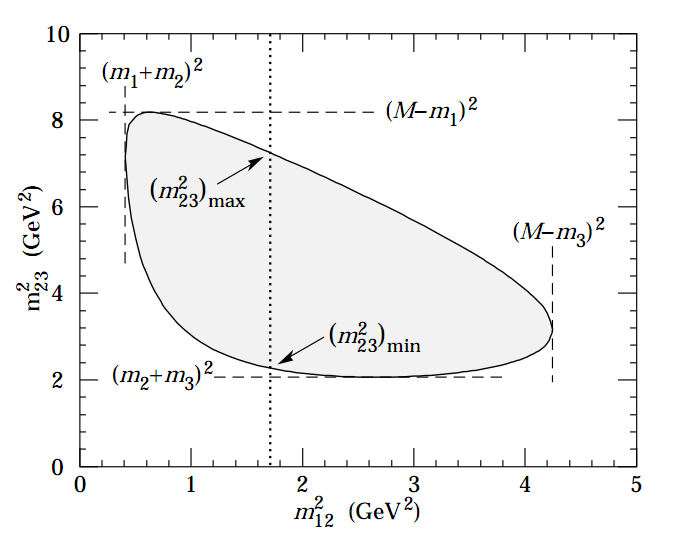
\includegraphics[width=0.5\textwidth]{immagini/Dalitz.png}
	\caption{Esempio di Dalitz Plot.}
	\label{fig:Dalitz}
\end{figure}
Adesso manca di osservare che nelle variabili scelte l'elemento infinitesimo dello spazio delle fasi di può scrivere come:
\[
	dL_p = \frac{1}{32s} \ ds_{12} \ ds_{23} \ d\alpha \ d\left( \cos(\beta) \right) \ d\gamma 
.\] 

Questo risultato mostra che lo spazio delle fasi è uniformemente popolato nella zona permessa (piatto) se si utilizzano le variabili descritte.\\

Venendo al dunque si ha che, sperimentalmente, quando questo spazio non è uniformemente popolato si può dedurre che vi sia un processo intermedio non previsto: un decadimento a due corpi in cui uno dei prodotti decade a sua volta in cue corpi, si hanno allora degli addensamenti nello spazio delle fasi in zone che ci indicano la massa invariante della particella instabile (dal decadimento a due). Questo è il metodo della massa invariante.



